\section{Event characterization}
\label{secks:eventchar}

The first analyses of LHC heavy-ion data dealt with the charged particle density and the energy density achieved in Pb--Pb interactions at an unprecedent collision energy of $\sqrt{s_{\rm NN}} = 2.76$~TeV per nucleon pair in centre-of-mass system. The estimated values, as well as the results of practically all other measurements, strongly depend on the geometry of the collision (also called centrality), more precisely on the distance $b$ of the centres of colliding nuclei in the plane transverse to the beam axis, called impact parameter of the collision. The impact parameter determines the volume of the interaction region, i.e. how violent the collision was.
%how many nucleons from the incoming nuclei actually took part in the collision
In this section we first describe how the centrality of Pb--Pb collisions is determined, and then we turn to the basic measurements which characterize these interactions at the LHC.



\subsection{Centrality determination}
\label{subsecks:centrality}

The lead nuclei are relatively extended objects, their size is about 14~fm across. To classify events according what part of the two nuclei participated in the interaction, the concept of collision centrality is commonly introduced in the field of heavy-ion physics. The centrality of the collision can be expressed in terms of geometrical parameters, such as the impact parameter $b$, or the number of participating nucleons. These parameters are inferred by comparison of experimental data with simulations of interactions. In this context the geometrical Glauber model is typically used~\cite{Miller:2007ri}, based on a description of pA and A--A scattering, originally proposed by R.J.~Glauber~\cite{Glauber:1955qq,Glauber:2006gd}. For the event simulation a Monte Carlo implementation of Glauber model is exploited~\cite{Shor:1988vk,Alver:2008aq}, which is realized by the following steps:
\begin{itemize}
    \item{randomly sample the position of each nucleon inside the nucleus according to a Woods--Saxon distribution (two-parameter Fermi distribution), using the parameters extracted from the analysis of low-energy elastic e--A scattering~\cite{DeJager:1987qc};}
    \item{randomly sample the collision impact parameter $b$ with probability distribution $P(b) \propto b \, {\rm d}b$ (up to $b_{\rm max} = 20$~fm, i.e. well above the lead nucleus diameter);}
    \item{assuming nucleons are moving along straight lines parallel to the beam direction, a pair of nucleons is considered as colliding if their centres are closer than $\sqrt{\sigma_{\rm NN}/\pi}$ in the transverse plane, where $\sigma_{\rm NN} = (64 \pm 5)$~mb is the inelastic nucleon--nucleon cross section, estimated from LHC pp measurements;}
\end{itemize}
and for each event the number of nucleons participating in at least one collision ($N_{\rm part}$) and the number of these binary collisions ($N_{\rm coll}$) are counted. Then the total nuclear Pb--Pb cross section ($\sigma_{\rm PbPb}$) is calculated as the fraction of $\pi b_{\rm max}^2$ given by the ratio of the number of events with $N_{\rm coll} \geq 1$ to the number of all generated events. The cross section for collisions with impact parameter in the interval $(0, b)$ is obtained the same way, counting the events with $N_{\rm coll} \geq 1$ having the impact parameter within that interval. The centrality for this impact-parameter selection is its cross section expressed as the percentage of $\sigma_{\rm PbPb}$. A centrality class is defined by its lower and upper percentages, corresponding to the events within impact-parameter interval $(b_{\rm l}, b_{\rm u})$, where the lower percentage is the part of $\sigma_{\rm PbPb}$ up to the impact parameter $b_{\rm l}$ and the upper percentage is that part up to $b_{\rm u}$. Other characterizations of centrality classes, such as the mean number of participants $\langle N_{\rm part} \rangle$ and the mean number of binary collisions $\langle N_{\rm coll} \rangle$ (obtained as the average values for events within that class) are also employed. For completeness, the geometrical overlap function (integral of the convolution  of the two transverse nuclear densities in the overlapping region) in the Monte Carlo formulation of Glauber model is defined as $T_{\rm AA} = N_{\rm coll} / \sigma_{\rm NN}$.

However, none of the geometrical quantities mentioned above ($b$, $N_{\rm part}$, $N_{\rm coll}$) is directly measurable in an experiment. Therefore, an experimental observable, which strongly correlates with the collision impact parameter, has to be used to classify the events according to their centrality. For example, the charged-particle multiplicity $N_{\rm ch}$ (or the energy deposition in a calorimeter) within a given pseudorapidity region is often used. In what follows the centrality determination as implemented by the ALICE collaboration is described~\cite{Abelev:2013qoq}, and later the differences for other experiments are mentioned. The centrality selection of events within a certain impact-parameter interval is then replaced by a selection using a $N_{\rm ch}$ interval. In an ideal case, if one were able to measure the event distribution in such new selection variable for all Pb--Pb nuclear collisions, it would be possible to define centrality selection and centrality percentiles without any model, using only this distribution and its integral. However, for very peripheral collisions (large $b$, low $N_{\rm ch}$) the experimental event sample is contaminated by electromagnetic interactions, at LHC energies these processes have  a huge cross section (more than two orders of magnitude larger than the nuclear cross section) and contribute to low multiplicity events~\cite{Bruce:2009bg,ALICE:2012aa}. It is necessary to suppress them, at least partly, already during the data taking (triggering on a minimum multiplicity value, or requiring some signal in ZDC's, see Sec.~\ref{subsecall:detectors}), which inevitably makes the event trigger less efficient for very peripheral collisions. For these reasons, the event distribution in a variable such as $N_{\rm ch}$ is usable for centrality selection only above some value, typically excluding peripheral collisions corresponding to the centrality class 90--100\,\%, where the contamination and the trigger inefficiency cannot be neglected. In order to determine the value, from which the distribution can be used, and to relate this so-called anchor point to the centrality, two approaches are utilized. The simulation of the Pb--Pb electromagnetic processes together with the experiment's trigger response gives the possibility to correct the event distribution of the selection variable, and to estimate a reasonable position of the anchor point with its centrality. Alternatively, the Glauber Monte Carlo can be supplemented with a model of particle production, describing the experimental selection-variable distribution and finding the point where the two deviate. Such an approach also allows to calculate for a given centrality selection the corresponding $\langle N_{\rm part} \rangle$ and $\langle N_{\rm coll} \rangle$, taking into account the finite resolution of the selection variable $N_{\rm ch}$ with respect to the collision impact parameter $b$.

A simple model for multiplicity production, exploited together with a Glauber Monte Carlo, consists in the simulation of the multiplicity distribution from one particle source and a prescription for the number of particle sources depending on the collision geometry, called the number of ancestors ($N_{\rm anc}$). For the multiplicity distribution the Negative Binomial Distribution (NBD) is typically used, it has two parameters (controlling the mean and width), and describes reasonably well the charged-particle multiplicity in different pseudorapidity windows for high-energy pp interactions. The number of particle sources is parameterized as a function of $N_{\rm part}$ and $N_{\rm coll}$, the common choice being $N_{\rm anc} = f N_{\rm part} + (1 - f) N_{\rm coll}$, motivated by a two-component model, where the number of sources is composed of soft (proportional to $N_{\rm part}$) and hard (proportional to $N_{\rm coll}$) interactions. Thus, such a model has three parameters, two for the NBD and $f$ for $N_{\rm anc}$, which are fitted to the experimental distribution of the selection variable between the anchor point and the maximal value (most central collisions).

\begin{figure}
\centering
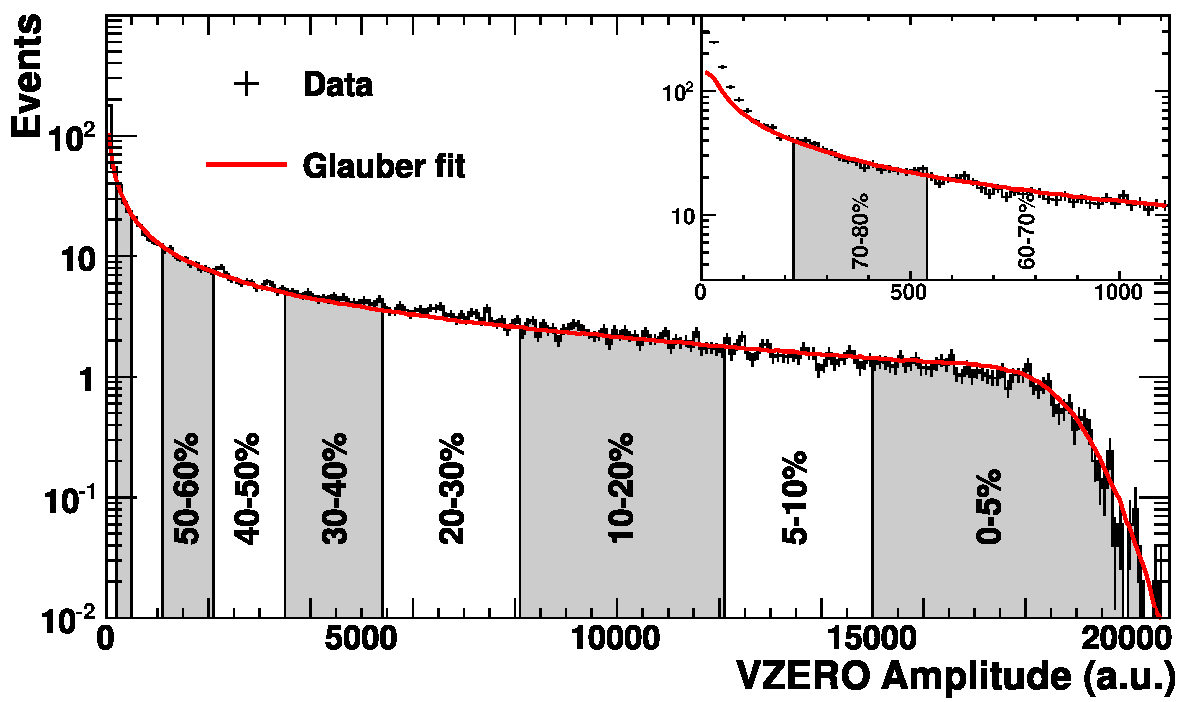
\includegraphics[width=0.5\textwidth]{ksfigures/VZEROCent.pdf}
\caption{Distribution of the sum of amplitudes from the VZERO scintillators in the ALICE experiment (histogram) fitted to Glauber Monte Carlo coupled to NBD multiplicity production model (line). The inset shows peripheral-collision region enlarged. Reproduced from~\cite{Abelev:2013qoq}.}
\label{figks:V0centr}
\end{figure}

Figure~\ref{figks:V0centr} illustrates the result of such a fit to the event distribution of the sum of amplitudes from the VZERO counters (see Sec.~\ref{subsecall:detectors} for detector description) in the ALICE detector. This variable is proportional to the multiplicity in the pseudorapidity region covered by the VZERO detector. The centrality classes and their percentiles are determined by integrating the experimental distribution from its maximal value down to the anchor point. Simulated events are then used to calculate $\langle N_{\rm part} \rangle$ and $\langle N_{\rm coll} \rangle$ for the centrality classes. The ATLAS experiment for the centrality selection is using transverse energy measured in Forward Calorimeters (FCal) and, instead of the model for multiplicity production, the pile-up of calorimeter response from $N_{\rm anc}$ pp collisions is exploited~\cite{ATLAS:2011ag}. The CMS experiment bases its Pb--Pb centrality selection on Hadron Forward (HF) calorimeter, and the distribution of the transverse-energy sum is corrected with the simulation of the trigger response~\cite{Chatrchyan:2011pb}. Another detector commonly used for centrality measurements is the ZDC. Its disadvantage is that, unlike for the multiplicity-type detectors, the ZDC response is not a monotonic function of centrality: it gives small signals both for very central and for very peripheral collisions. ZDC's are therefore normally used in correlation with some other detector, especially for central and very central events.

The centrality determination and its uncertainties affect practically all the results from the analyses of heavy-ion data. A careful systematic study of the centrality selection dependence on different assumptions is always required. This usually includes: variation of the parameters describing the nucleus density; including or not a minimal separation between nucleons inside each nucleus; modifying the definition of colliding nucleons (from a black-disc assumption to a Gaussian profile description, or introducing an intra-nuclear rescattering); and changing the functional dependence of $N_{\rm anc}$, if used, to a power function of $N_{\rm part}$ or $N_{\rm coll}$. All these uncertainties must then be properly propagated to the measurements of other quantities.

\subsection{Charged-particle density}
\label{subsecks:partdensity}
Traditionally, the very first measurements of heavy-ion collisions at a new energy regime comprise the charged-particle density, and its centrality dependence. These measurements were performed by all three experiments participating in the LHC heavy-ion programme~\cite{Aamodt:2010pb,Aamodt:2010cz,ATLAS:2011ag,Chatrchyan:2011pb}, and the first results were published already during the first heavy-ion run~\cite{Aamodt:2010pb}. The methods exploited to measure the charged-particle density (${\rm d}N_{\rm ch}/{\rm d}\eta$) in the mid-rapidity region ($|\eta| < 0.5$) were very similar. All experiments used their silicon pixel trackers, detectors closest to the interaction point, to count so called tracklets, pairs of reconstructed hits (pixel clusters) in two layers of the pixel detectors aligned with the primary vertex. Other methods, such as measuring the cluster multiplicity, partial tracking with innermost detectors, and TPC tracking (in the case of ALICE), were also utilized. The collision-energy dependence of ${\rm d}N_{\rm ch}/{\rm d}\eta$ for the most central heavy-ion collisions, normalized per participant pair (i.e. $\langle N_{\rm part} \rangle /2$), is presented in Fig.~\ref{figks:EnrgyMult}, top part. The results from the three experiments are in excellent agreement, and they show an increase by more than factor of two, compared to the highest value observed at RHIC. The energy dependence of the charged-particle density can be satisfactorily parameterized by a power function: $\propto s_{\rm NN}^{0.15}$. Note that the energy dependence for heavy ions is significantly steeper than that for pp interactions ($\propto s^{0.11}$), this is also reflected by the more than a factor two higher value of the normalized charged-particle density $({\rm d}N_{\rm ch}/{\rm d}\eta)/(0.5\langle N_{\rm part} \rangle)$ in heavy-ion collisions compared to pp interactions. It is interesting to note that most of the theoretical and model predictions for the LHC charged-particle density underestimated the experimental observation~\cite{Aamodt:2010pb}, contrary to a clear tendency for an overestimation when the first results from RHIC experiments were published.

\begin{figure}
\centering
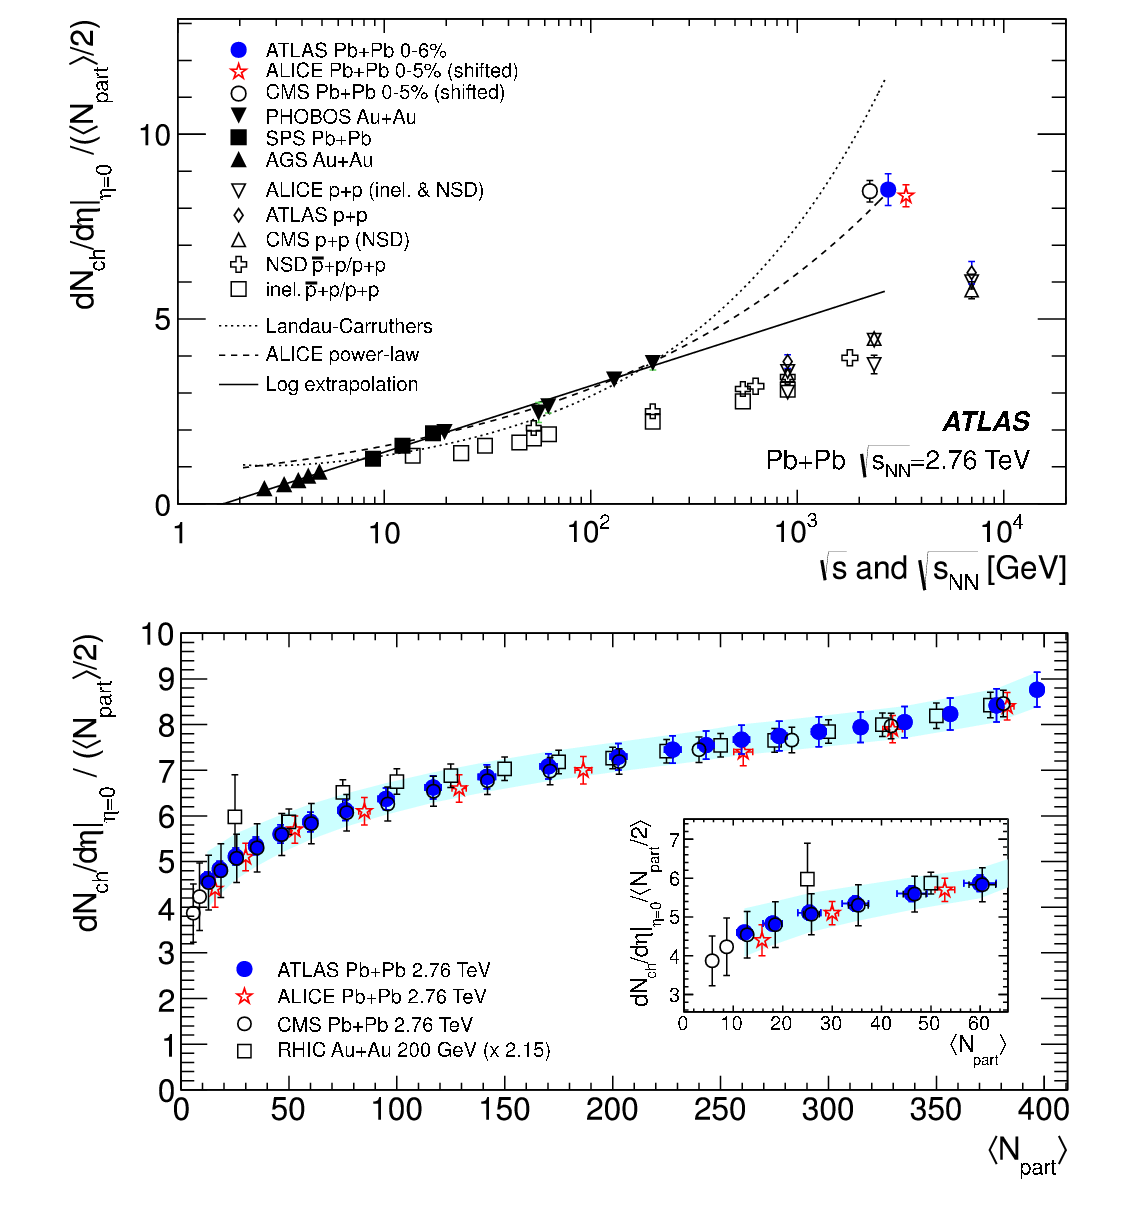
\includegraphics[width=0.5\textwidth]{ksfigures/EnergCentMult.png}
\caption{Top: Energy dependence of the charged-particle density at mid-rapidity ($|\eta| < 0.5$) normalized per participant nucleon pair, from various pp (and $\overline{\rm p}$p) measurements, and most central heavy-ion collisions. The curves represent various extrapolations from lower-energy data to LHC, the one describing heavy-ion experimental points (dashed line) is a power function $({\rm d}N_{\rm ch}/{\rm d}\eta)/(0.5 \langle N_{\rm part} \rangle) \propto s_{\rm NN}^{0.15}$ proposed in~\cite{Aamodt:2010pb}. Bottom: $\langle N_{\rm part} \rangle$ dependence of the charged-particle density normalized per participant nucleon pair from the three LHC experiments, compared to average value from RHIC experiments, multiplied by a factor $2.15$. The inset shows in detail the peripheral-collision region with $\langle N_{\rm part} \rangle < 60$. Reproduced from~\cite{ATLAS:2011ag}.}
\label{figks:EnrgyMult}
\end{figure}

In the bottom part of Fig.~\ref{figks:EnrgyMult} the centrality dependence of the same quantity $({\rm d}N_{\rm ch}/{\rm d}\eta)/(0.5 \langle N_{\rm part} \rangle)$, expressed as a function of $\langle N_{\rm part} \rangle$, is presented. Again, very good agreement among the three LHC experiments is observed. The data from RHIC (average value over the four experiments~\cite{Adler:2004zn}) are also shown, multiplied by a factor $2.15$ to match the points for the most central collisions. The normalized charged-particle density is rising with centrality, which means that the particle multiplicity at mid-rapidity increases faster than the number of participants, presumably due to the contribution of hard processes to the multiplicity production. However, this increase is very similar to that observed at the top RHIC energy. Apart from a simple interpretation of these data in terms of (a mixture of) soft and hard interactions, model calculations implementing a saturation picture, where the number of soft gluons available for the multiplicity production is progressively reduced by parton recombination, attempt to determine the energy and centrality dependence of the saturation scale~\cite{Armesto:2004ud,Kharzeev:2004if,ALbacete:2010ad}.

The experiments were also looking for the ${\rm d}N_{\rm ch}/{\rm d}\eta$ evolution in the longitudinal direction, i.e. as a function of pseudorapidity. The ATLAS collaboration published the charged-particle densities for different centrality classes in $|\eta| < 2$~\cite{ATLAS:2011ag}, and the CMS detector measured ${\rm d}N_{\rm ch}/{\rm d}\eta$ in the interval $|\eta| < 2.5$~\cite{Chatrchyan:2011pb}. The ALICE experiment extended the pseudorapidity coverage of such measurement to $- 5 < \eta < 5.5$~\cite{Abbas:2013bpa}, exploiting the FMD (see Sec.~\ref{subsecall:detectors}) and so called satellite bunches. The latter are created in the accelerator RF cavities, when a small fraction of particles slips from the main bunch into another wave period, $75$~cm apart (corresponding to RF frequency $400$~MHz). This way, very low-intensity satellite collisions, distanced by every $37.5$~cm from the main bunch crossing, are produced, shifting the pseudorapidity acceptance. Figure~\ref{figks:MultEta} shows the results of the ALICE pseudorapidity distribution measurement, compared to the data previously obtained by CMS and ATLAS. The wide-rapidity data are used together with the RHIC results (from the BRAHMS~\cite{Bearden:2001qq} and PHOBOS~\cite{Alver:2010ck} experiments) to confirm limiting fragmentation --- the shape of the distributions are in the fragmentation region independent of the collision energy. By extrapolation, the total charged-particle multiplicity in Pb--Pb collisions at $\sqrt{s_{\rm NN}} = 2.76$~TeV for different centralities can be estimated, for example, in 5\,\% of the most central events $(17.2 \pm 0.8) \times 10^3$ charged particles are created.

\begin{figure}
\centering
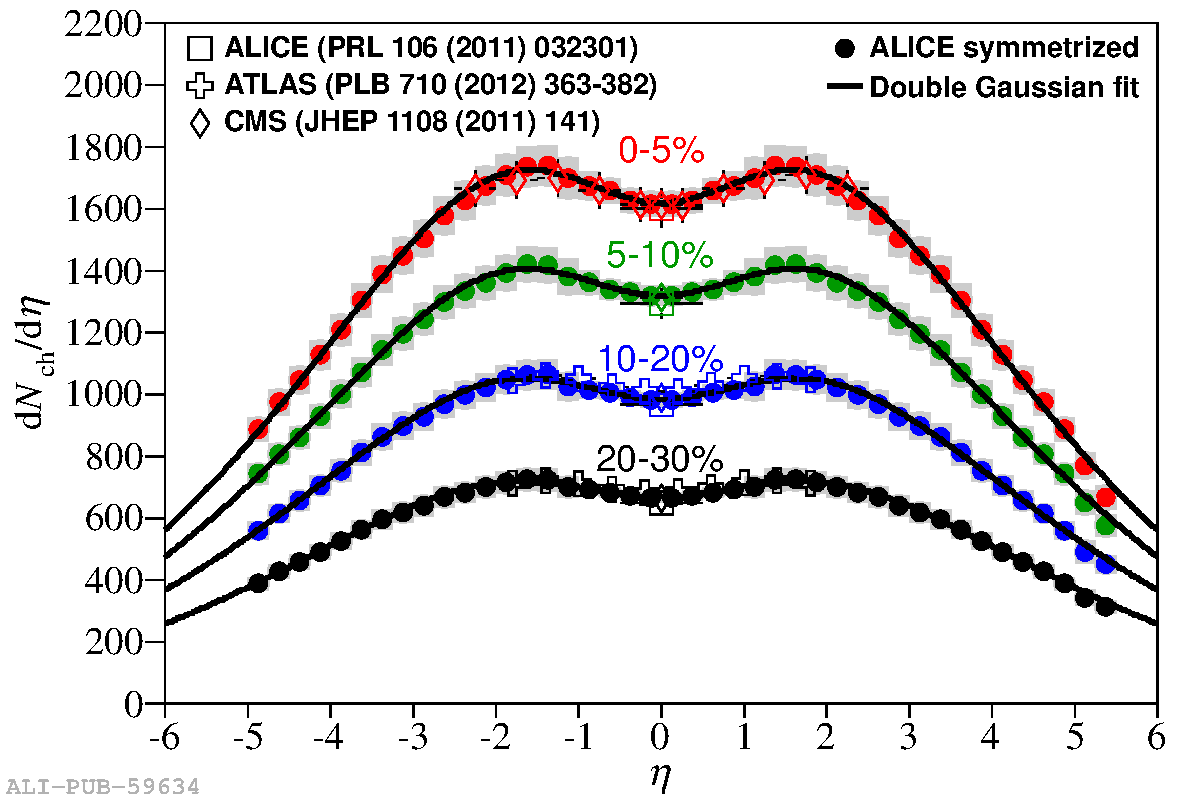
\includegraphics[width=0.5\textwidth]{ksfigures/MultEtaCent.pdf}
\caption{Charged-particle pseudorapidity density distribution for various centrality classes, comparison among the LHC experiments. Reproduced from~\cite{Abbas:2013bpa}.}
\label{figks:MultEta}
\end{figure}


%charged particle density vs energy
%charged particle density vs centrality
%charged particle density vs pseudorapidity
\subsection{Energy density}
\label{subsecks:energydensity}

In order to estimate the energy density achieved in Pb--Pb collisions at the LHC, the measurements of the transverse energy pseudorapidity density, ${\rm d}E_{\rm T}/{\rm d}\eta$ were performed. The CMS experiment measured directly the energy flow in calorimeters for different pseudorapidities and centralities~\cite{Chatrchyan:2012mb}. The collision energy dependence of ${\rm d}E_{\rm T}/{\rm d}\eta$ at mid-rapidity for the most central heavy-ion collisions, normalized to the the number of participant pairs, is shown in Fig.~\ref{figks:ETvsEnerg}. An increase by more than a factor three is observed from the top RHIC energy to the LHC. This collision-energy dependence can be satisfactorily described by a power function $\propto s_{\rm NN}^{0.2}$, which means that the transverse-energy density rises with collision energy faster than the particle density, indicating a significant increase of the average transverse momentum of particles produced in the LHC heavy-ion interactions. The ALICE experiment confirmed the CMS results estimating ${\rm d}E_{\rm T}/{\rm d}\eta$ from ${\rm d}N_{\rm ch}/{\rm d}\eta$ and the measured transverse-momentum spectra for different hadron species.

\begin{figure}
\centering
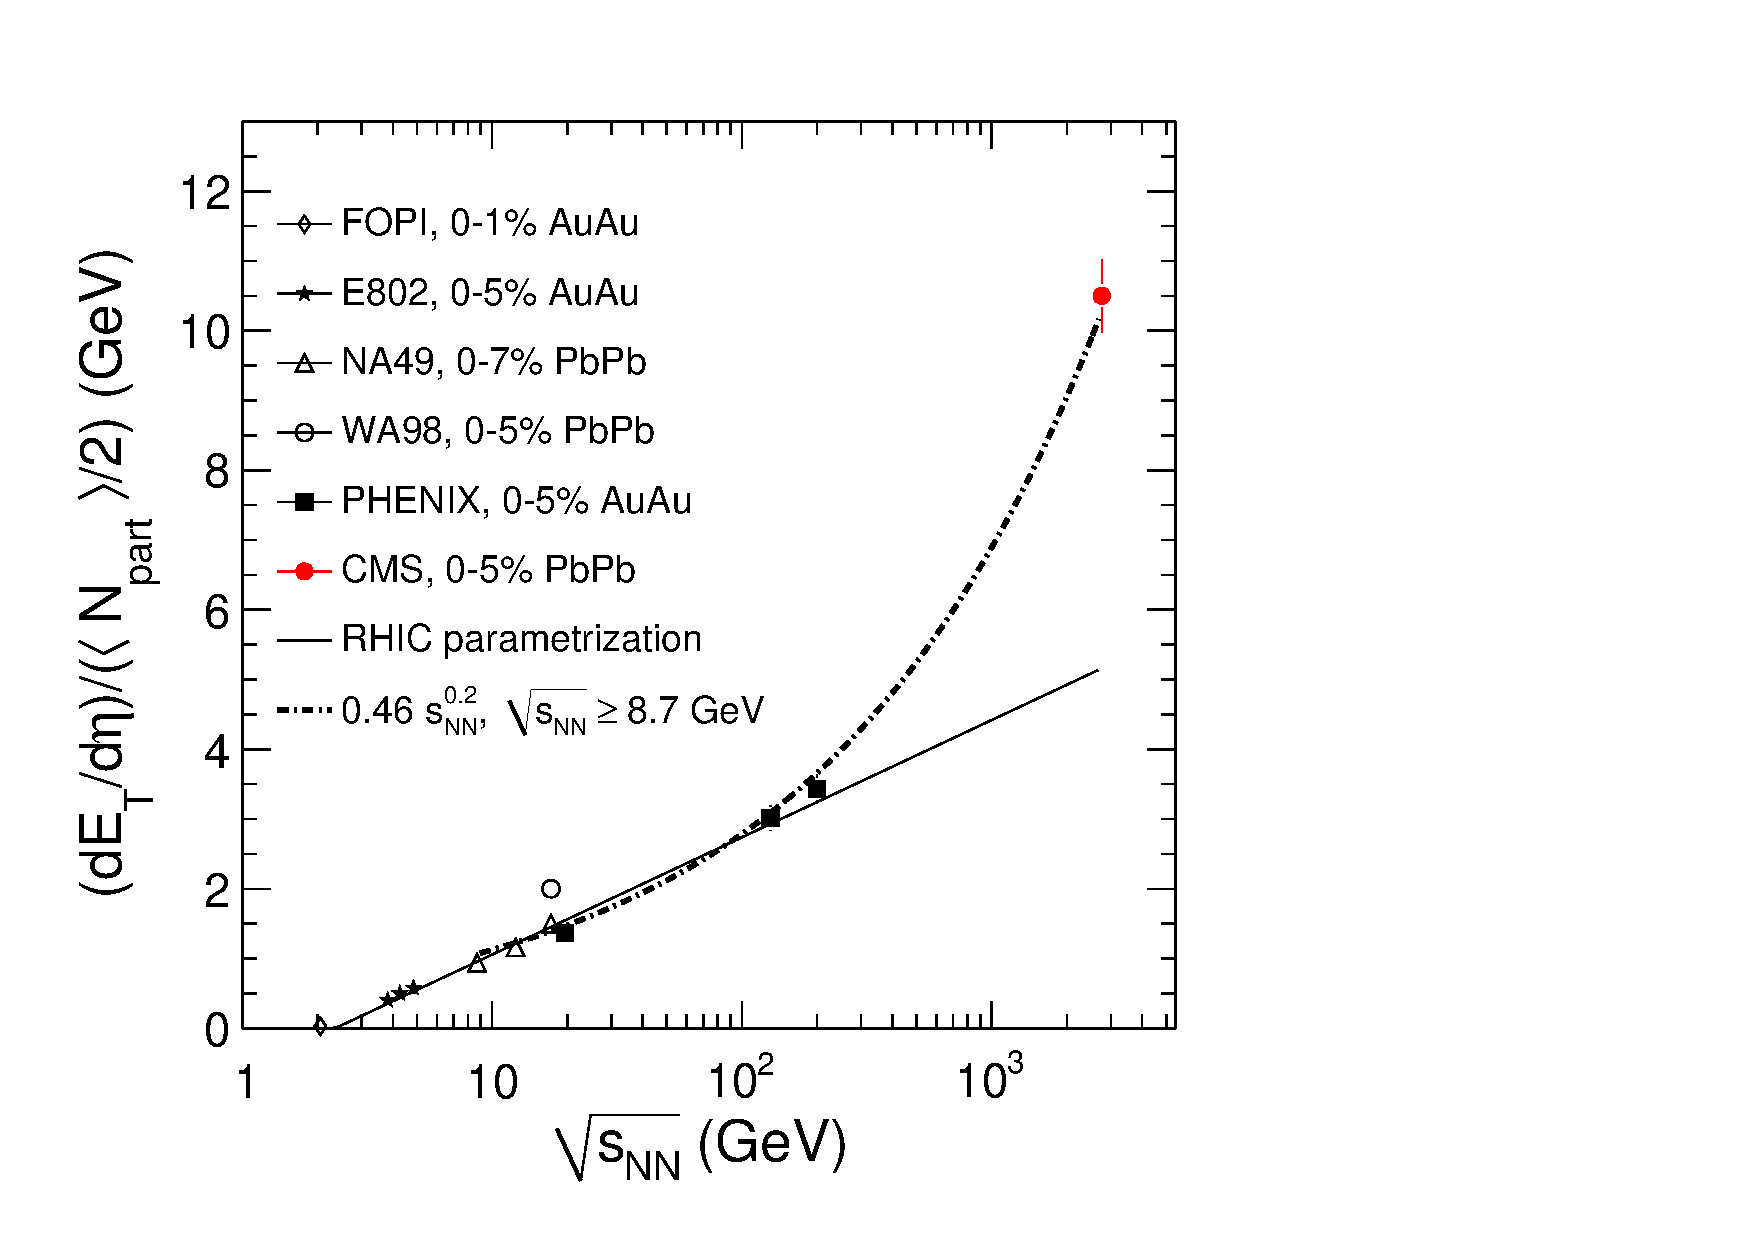
\includegraphics[width=0.5\textwidth]{ksfigures/CMSETvsEnerg.pdf}
\caption{Collision energy dependence of the transverse-energy pseudorapidity density at mid-rapidity, normalized to the number of participant pairs, for central heavy-ion collisions. The curves represent various extrapolations from lower-energy data to LHC, the one describing the LHC measurement (dashed--dotted line) is a power function $({\rm d}E_{\rm T}/{\rm d}\eta)/(0.5 \langle N_{\rm part} \rangle) \propto s_{\rm NN}^{0.2}$ proposed in~\cite{Chatrchyan:2012mb}, from where this figure is reproduced.}
\label{figks:ETvsEnerg}
\end{figure}

Even in forward region, up to $|\eta| = 5$, the transverse-energy density observed at the LHC is larger than that at mid-rapidity at the top RHIC energy. The energy density achieved in heavy-ion interactions ($\epsilon$) is commonly related to the transverse-energy density by the Bjorken formula~\cite{Bjorken:1982qr}, based on geometrical considerations. It can be expressed as $\epsilon \tau_{0} = ({\rm d}E_{\rm T}/{\rm d}y) / S$, where $\tau_{0}$ denotes the time when the initial thermalization was established (supposed to be $\tau_{0} \leq 1$~fm), and $S$ is the transverse overlap area, approximated for central Pb--Pb collisions with $\pi (7\,{\rm fm})^2$. For the top 5\,\% centrality CMS obtained $\epsilon \tau_{0} = 14$~GeV/fm$^2$ (using a model estimation for Jacobian ${\rm d}\eta/{\rm d}y \approx 1.1$). This represents a factor 2.6 increase with respect to the highest RHIC collision energy, and an even larger increase for the energy density $\epsilon$, since the time $\tau_{0}$ is expected to be shorter at the LHC.
%energy density vs energy
